%%%%%%%%%%%%%%%%%%%%%%%%%%%%%%%%%%%%%%%%%
% Beamer Presentation
% LaTeX Template
% Version 1.0 (10/11/12)
%
% This template has been downloaded from:
% http://www.LaTeXTemplates.com
%
% License:
% CC BY-NC-SA 3.0 (http://creativecommons.org/licenses/by-nc-sa/3.0/)
%
%%%%%%%%%%%%%%%%%%%%%%%%%%%%%%%%%%%%%%%%%

%-------------------------------------------------------------------------------
%	PACKAGES AND THEMES
%-------------------------------------------------------------------------------

\documentclass{beamer}
\usepackage{xcolor}
\usepackage{graphicx}
\usepackage{tikz}
\usepackage{listings}
\usepackage{multicol}
\usepackage{listings-rust}

\DeclareMathOperator{\diag}{diag}

\definecolor{applegreen}{rgb}{0.55, 0.71, 0.0}
\definecolor{blue(ncs)}{rgb}{0.0, 0.45, 0.60}
\definecolor{burgundy}{rgb}{0.5, 0.0, 0.13}

\definecolor{cadet}{rgb}{0.33, 0.41, 0.47}
\definecolor{airforceblue}{rgb}{0.36, 0.54, 0.66}

\mode<presentation> {

\usetheme{CambridgeUS}

\usecolortheme{wolverine}

\definecolor{gold}{HTML}{D4A017}
\definecolor{darkgold}{HTML}{B7950B}

\setbeamercolor{palette primary}{bg=cadet,fg=white}
\setbeamercolor{palette secondary}{bg=airforceblue,fg=white}
\setbeamercolor{palette tertiary}{bg=black,fg=white}
\setbeamercolor{palette quaternary}{bg=cadet,fg=white}

\setbeamercolor{frametitle}{bg=airforceblue,fg=white}

\setbeamercolor{section number projected}{bg=black,fg=cadet}
\setbeamercolor{item}{fg=black,bg=cadet}

\setbeamertemplate{page number in head/foot}[framenumber]
}

\usepackage{lmodern}

\lstdefinestyle{colouredC}{ 
  commentstyle=\color[gray]{0.4},
  keywordstyle=\bfseries,
  keywordstyle=[2]\color[rgb]{0.75, 0, 0},
  keywordstyle=[3]\color[rgb]{0, 0.5, 0},
  keywordstyle=[4]\color[rgb]{0, 0.5, 0},
  keywordstyle=[5]\color[rgb]{0, 0, 0.75},
  numberstyle=\tiny\color{mGray},
  stringstyle=\color[rgb]{0, 0, 0.5},
  basicstyle=\ttfamily,
  language=C,
  morekeywords=[3]{CeedInt, CeedScalar},
}

\lstdefinestyle{boxedC}{
  style=colouredC,
  numbers=left,
  firstnumber=auto,
  numberblanklines=true,
  frame=trbL,
  numberstyle=\tiny,
  frame=leftline,
  numbersep=7pt,
  framesep=5pt,
  framerule=10pt,
  xleftmargin=15pt,
  backgroundcolor=\color[gray]{0.97},
  rulecolor=\color[gray]{0.90}%
}

\lstdefinelanguage{TOML}{
  keywords={typeof, new, true, false, catch, function, return, null, catch, switch, var, if, in, while, do, else, case, break},
  ndkeywords={class, export, boolean, throw, implements, import, this},
  sensitive=false,
  comment=[l]{//},
  morecomment=[s]{/*}{*/},
  morestring=[b]',
  morestring=[b]",
  columns=spaceflexible,
}

\lstdefinestyle{boxedTOML}{
  language=TOML,
  numbers=left,
  firstnumber=auto,
  numberblanklines=true,
  frame=trbL,
  numberstyle=\tiny,
  frame=leftline,
  numbersep=7pt,
  framesep=5pt,
  framerule=10pt,
  xleftmargin=15pt,
  backgroundcolor=\color[gray]{0.97},
  rulecolor=\color[gray]{0.90}
}

\lstdefinestyle{boxedSH}{
  language=sh,
  numbers=left,
  firstnumber=auto,
  numberblanklines=true,
  frame=trbL,
  numberstyle=\tiny,
  frame=leftline,
  numbersep=7pt,
  framesep=5pt,
  framerule=10pt,
  xleftmargin=15pt,
  backgroundcolor=\color[gray]{0.97},
  rulecolor=\color[gray]{0.90}%
}

\lstdefinelanguage{makefile}{
  keywords={typeof, new, true, false, catch, function, return, null, catch, switch, var, if, in, while, do, else, case, break},
  ndkeywords={class, export, boolean, throw, implements, import, this},
  sensitive=false,
  comment=[l]{\#},
  morestring=[b]',
  morestring=[b]",
  columns=spaceflexible,
}

\lstdefinestyle{boxedMakefile}{
  language=makefile,
  numbers=left,
  firstnumber=auto,
  numberblanklines=true,
  frame=trbL,
  numberstyle=\tiny,
  frame=leftline,
  numbersep=7pt,
  framesep=5pt,
  framerule=10pt,
  xleftmargin=15pt,
  backgroundcolor=\color[gray]{0.97},
  rulecolor=\color[gray]{0.90}%
}

\usepackage{graphicx} % Allows including images
\usepackage{booktabs} % Allows the use of \toprule, \midrule and \bottomrule in tables

%-------------------------------------------------------------------------------
%	TITLE PAGE
%-------------------------------------------------------------------------------

\title[Rust for HPC]{Productive Performance Portability: Building in Rust with PETSc and libCEED} % The short title appears at the bottom of every slide, the full title is only on the title page

\author{Jeremy L Thompson} % Your name
\institute[CU Boulder] % Your institution as it will appear on the bottom of every slide, may be shorthand to save space
{University of Colorado Boulder \\ % Your institution for the title page
\medskip
\textit{jeremy@jeremylt.org} % Your email address
}
\date{23 Feburary 2022} % Date, can be changed to a custom date

\begin{document}

\begin{frame}
\titlepage % Print the title page as the first slide
\end{frame}

%-------------------------------------------------------------------------------

\begin{frame}
\begin{center}
\frametitle{Funding}

The authors acknowledge support by the Department of Energy, National Nuclear Security Administration, Predictive Science Academic Alliance Program (PSAAP) under Award Number DE-NA0003962.

\end{center}
\end{frame}
 
%-------------------------------------------------------------------------------

\begin{frame}
\frametitle{Overview} % Table of contents slide, comment this block out to remove it
\tableofcontents % Throughout your presentation, if you choose to use \section{} and \subsection{} commands, these will automatically be printed on this slide as an overview of your presentation
\end{frame}

%-------------------------------------------------------------------------------
%	PRESENTATION SLIDES
%-------------------------------------------------------------------------------

%-------------------------------------------------------------------------------
\section{Introduction}
%-------------------------------------------------------------------------------

\begin{frame}
\begin{center}
\frametitle{Rust for HPC}

\begin{itemize}

\item Rust provides high performance with modern tooling and ergonomic language features\\

~\\

\item We look at the libCEED and PETSc Rust wrappers\\

~\\

\item The libCEED wrapper provides performance portable matrix-free finite element operators\\

~\\

\item The PETSc wrapper is a more complex ongoing challenge\\

\end{itemize}

~\\

\bf{Rust is ready for HPC - but it requires rethinking your design!}

\end{center}
\end{frame}

%-------------------------------------------------------------------------------
\section{Why Rust?}
%-------------------------------------------------------------------------------

\begin{frame}
\begin{center}
\frametitle{Rust - Language features}

\begin{itemize}

\item Strongly typed language with a focus on performance and safety\\

~\\

\item Compile-time memory management via lifetimes\\

~\\

\item Borrow checker protects data, tracking ownership and access\\

~\\

\item Many C run-time bugs become Rust compile-time errors\\

\end{itemize}

\end{center}
\end{frame}

%-------------------------------------------------------------------------------

\begin{frame}
\begin{center}
\frametitle{Rust - Ergonomics}

\begin{itemize}

\item Installing - Cargo + crates.io manages dependencies vs Make\\

~\\

\item Abstractions - zero cost abstractions for high-level language features\\

~\\

\item Documentation - Automatic documentation with doctests using Cargo + docs.rs\\

~\\

\item Unit Tests - Doctests and unit tests integrated with Cargo\\

\end{itemize}

\end{center}
\end{frame}

%-------------------------------------------------------------------------------
\section{libceed-rs}
%-------------------------------------------------------------------------------

\begin{frame}
\begin{center}
\frametitle{libCEED Representation}

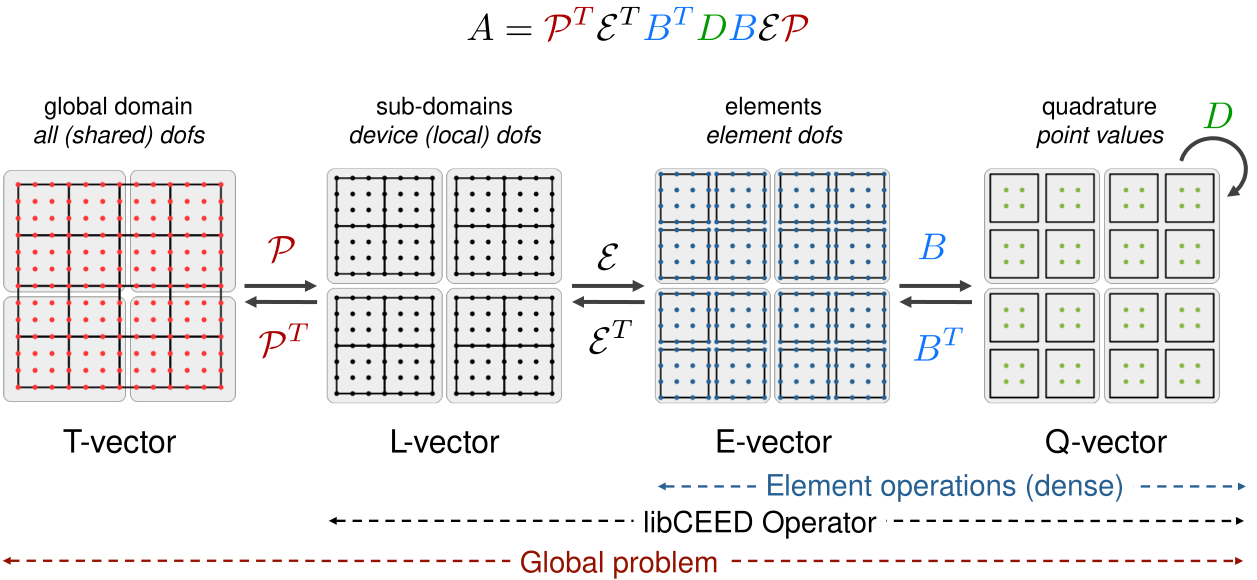
\includegraphics[height=4.5cm]{libCEEDAPI}\cite{libceed}

\begin{itemize}

\item ${\color{burgundy}\mathbf{P}}$ - parallel element assembly operator

\item $\mathbf{G}$ - local element assembly operator\\

\item ${\color{blue(ncs)}\mathbf{B}}$ - basis action operator\\

\item ${\color{applegreen}\mathbf{D}}$ - weak form and geometry at quadrature points\\

\end{itemize}

\end{center}
\end{frame}

%-------------------------------------------------------------------------------

\begin{frame}
\begin{center}
\frametitle{libCEED Backends}

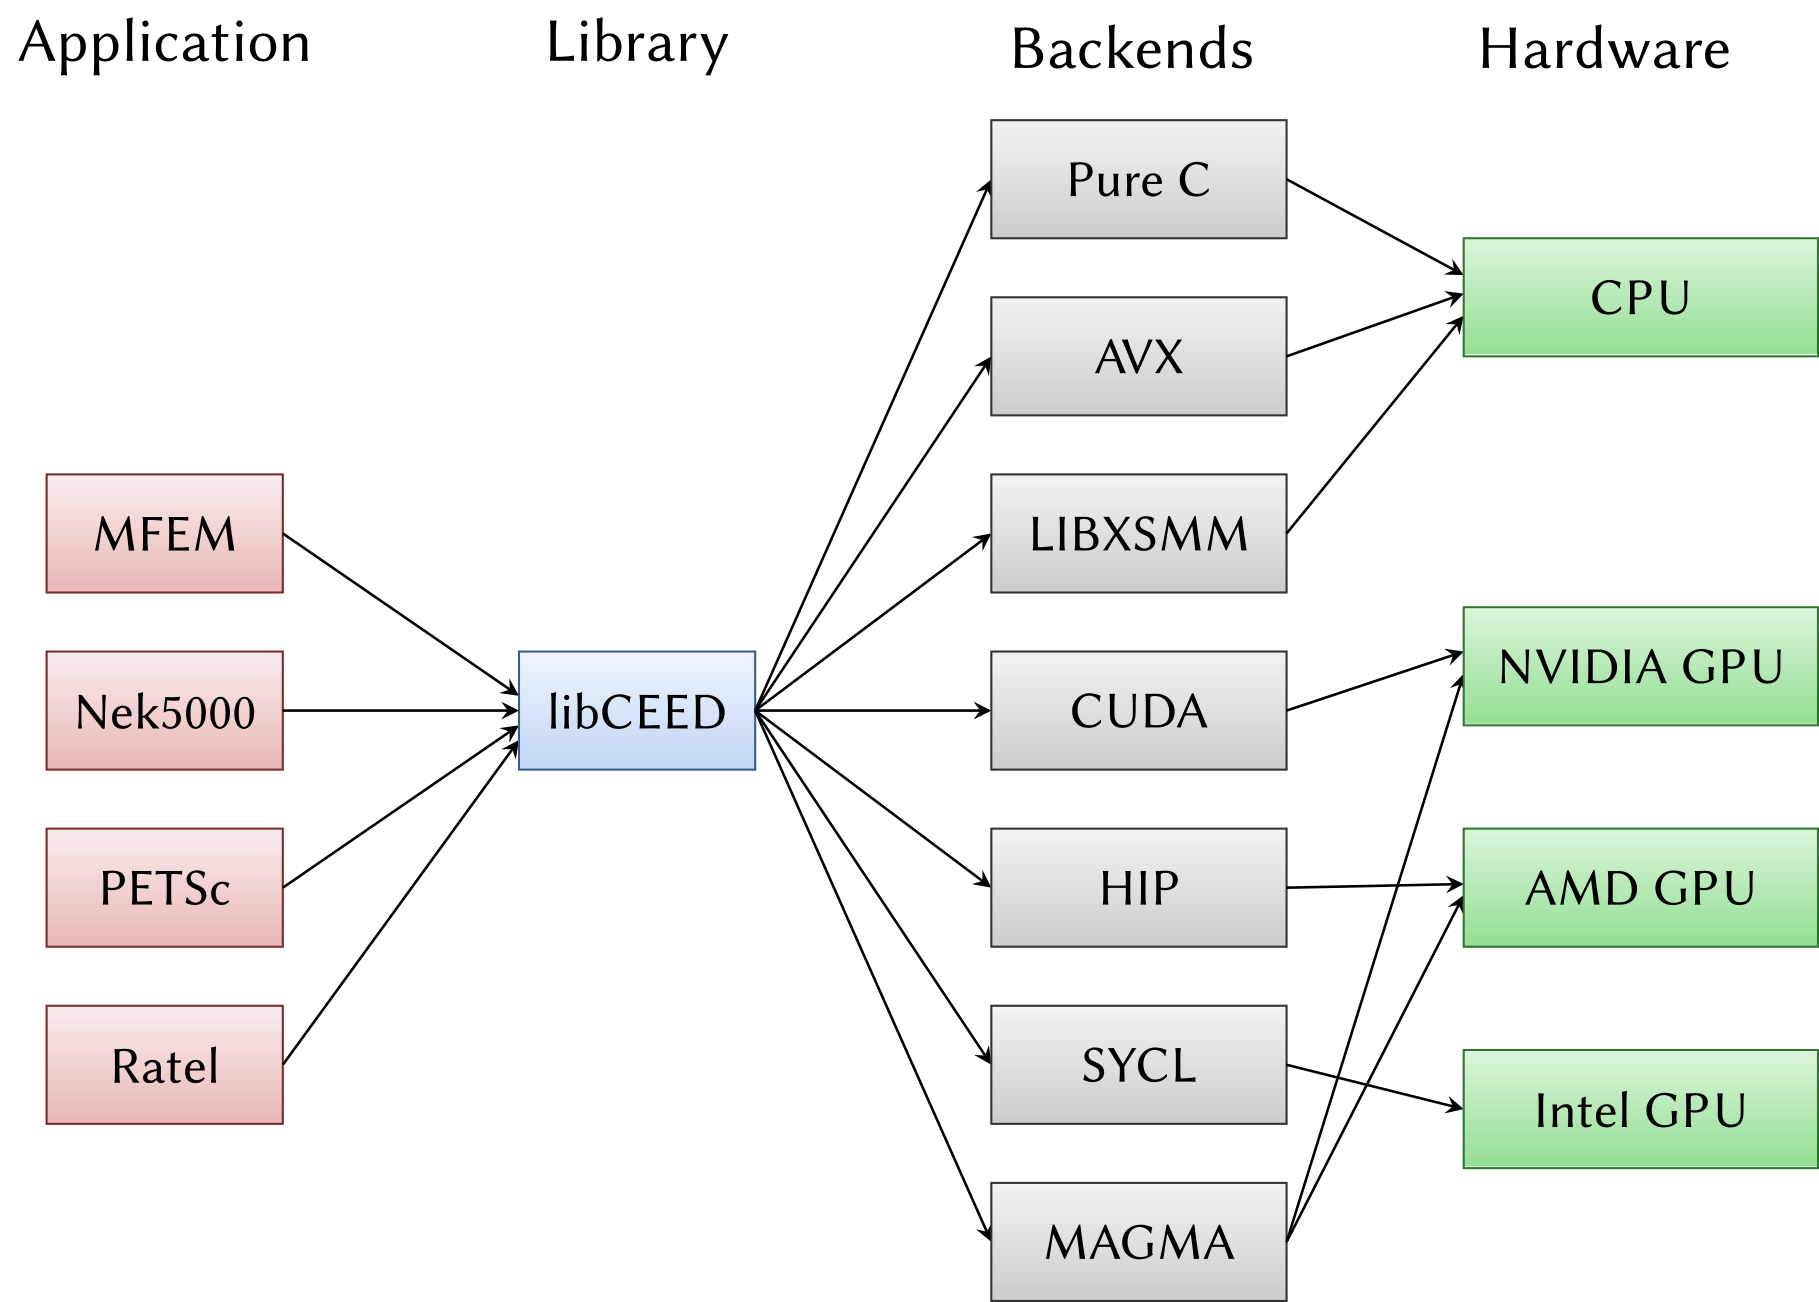
\includegraphics[height=5.5cm]{libCEEDBackends}\cite{libceed}

Multiple backends provide performance portability at runtime\\

~\\

Rust wrapper preserves this capabilty (mostly)!

\end{center}
\end{frame}

%-------------------------------------------------------------------------------

\begin{frame}[fragile]
\begin{center}
\frametitle{libceed-rs}

\href{https://lib.rs/crates/libceed}{https://lib.rs/crates/libceed}\\

\href{https://github.com/ceed/libceed}{https://github.com/ceed/libceed}\\

~\\

\begin{itemize}

\item Faithful translation of C API into Rust\\

~\\

\item Additional objects to help manage borrowed vector access\\

~\\

\item Currently no native Rust GPU QFunction support\\

\end{itemize}

~\\

{\footnotesize
\begin{lstlisting}[language=Rust, style=boxedRust]
extern crate libceed;
fn main() -> libceed::Result<()> {
    let ceed = libceed::Ceed::init("/cpu/self/ref");
    let u = ceed.vector_from_slice(&[0.0, 0.5, 1.0])?;
    let u_view = u.view()?;
    assert_eq!(u_view[..], [0.0, 0.5, 1.0]);
    Ok(())
}
\end{lstlisting}
}

\end{center}
\end{frame}

%-------------------------------------------------------------------------------

\begin{frame}[fragile]
\begin{center}
\frametitle{Building}

Building dependencies reliabily across platforms can be... painful\\

~\\

{\scriptsize
\begin{lstlisting}[language=makefile, style=boxedMakefile]
...

ifneq ($(wildcard $(XSMM_DIR)/lib/libxsmm.*),)
  PKG_LIBS += -L$(abspath $(XSMM_DIR))/lib -lxsmm -ldl
  MKL ?=
  ifeq (,$(MKL)$(MKLROOT))
    BLAS_LIB = -lblas
  else
    ifneq ($(MKLROOT),)
      # Some installs put everything inside subdirectory
      MKL_LIBDIR = $(dir $(firstword $(wildcard $(MKLROOT)/lib/intel64/libmkl_sequential.* $(MKLROOT)/lib/libmkl_sequential.*)))
      MKL_LINK = -L$(MKL_LIBDIR)
      PKG_LIB_DIRS += $(MKL_LIBDIR)
    endif
    BLAS_LIB = $(MKL_LINK) -Wl,--push-state,--no-as-needed -lmkl_intel_lp64 -lmkl_sequential -lmkl_core -lpthread -lm -ldl -Wl,--pop-state
  endif
  PKG_LIBS += $(BLAS_LIB)
endif
...
\end{lstlisting}
}

\end{center}
\end{frame}

%-------------------------------------------------------------------------------

\begin{frame}[fragile]
\begin{center}
\frametitle{Building}

Far simpler dependency specification for Rust!\\

~\\

{\footnotesize
\begin{lstlisting}[language=TOML, style=boxedTOML]
[package]
name = "ex1-volume"
version = "0.1.0"
authors = [
    "Jeremy L Thompson <thompson.jeremy.luke@gmail.com>",
]
edition = "2018"

[dependencies]
libceed = "0.9.0"
structopt = { version = "0.3", default-features = false }
mesh = { path = "../mesh" }
\end{lstlisting}
}

Easier building

{\footnotesize
\begin{lstlisting}[language=sh, style=boxedSH]
$ cargo build
\end{lstlisting}
}

\end{center}
\end{frame}

%-------------------------------------------------------------------------------

\begin{frame}[fragile]
\begin{center}
\frametitle{High Level Abstractions - User QFunctions}

User source for physics at quadrature points requires some additional boilerplate in C/CUDA single source\\

~\\

{\footnotesize
\begin{lstlisting}[language=C, style=boxedC]
CEED_QFUNCTION(MassApply)(void *ctx, const CeedInt Q,
                          const CeedScalar *const *in,
                          CeedScalar *const *out) {
  // Unpack input and output arrays
  const CeedScalar *u = in[0], *rho = in[1];
  CeedScalar *v = out[0];

  // Loop over all quadrature points
  CeedPragmaSIMD
  for (CeedInt i = 0; i < Q; i++) {
    v[i] = u[i] * rho[i];
  }

  return 0;
}
\end{lstlisting}
}

\end{center}
\end{frame}

%-------------------------------------------------------------------------------

\begin{frame}[fragile]
\begin{center}
\frametitle{High Level Abstractions - User QFunctions}

Rust inteface presents more clarity, less opportunity for error\\

~\\

{\footnotesize
\begin{lstlisting}[language=Rust, style=boxedRust]
// QFunction from user closure
let apply_mass = |
    [u, qdata, ..]: QFunctionInputs,
    [v, ..]: QFunctionOutputs,
| {
    // Protected array access!
    v.iter_mut()
        .zip(u.iter().zip(qdata.iter()))
        .for_each(|(v, (u, rho))| *v = u * rho);

    0
};
\end{lstlisting}
}

\end{center}
\end{frame}

%-------------------------------------------------------------------------------

\begin{frame}[fragile]
\begin{center}
\frametitle{Documentation}

Documentation and testing separate in C\\

Often multiple processing steps to generate documentation\\

~\\

{\footnotesize
\begin{lstlisting}[language=C, style=boxedC]
/**
  @brief Create a CeedVector of the specified length
           (does not allocate memory)

  @param      ceed   Ceed context
  @param      length Length of vector
  @param[out] vec    Address where the newly created
                       CeedVector will be stored

  @return An error code: 0 - success, otherwise - failure

  @ref User
**/
int CeedVectorCreate(Ceed ceed, CeedInt length,
                     CeedVector *vec) { /* */ };
\end{lstlisting}
}

\end{center}
\end{frame}

%-------------------------------------------------------------------------------

\begin{frame}[fragile]
\begin{center}
\frametitle{Documentation}

Integrated documentation and unit tests in Rust\\

~\\

{\footnotesize
\begin{lstlisting}[language=Rust, style=boxedRust]
/// Returns a Vector of the specified length
///   (does not allocate memory)
///
/// # arguments
///
/// * `n` - Length of vector
///
/// ```
/// # use libceed::prelude::*;
/// # fn main() -> libceed::Result<()> {
/// # let ceed = libceed::Ceed::default_init();
/// let vec = ceed.vector(10)?;
/// # Ok(())
/// # }
/// ```
pub fn vector<'a>(&self, n: usize) -> Result<Vector<'a>> { /* */ }
\end{lstlisting}
}

\end{center}
\end{frame}

%-------------------------------------------------------------------------------

\begin{frame}[fragile]
\begin{center}
\frametitle{Documentation}

Easier testing and documentation

{\footnotesize
\begin{lstlisting}[language=sh, style=boxedSH]
$ cargo test
$ cargo fmt
$ cargo doc
\end{lstlisting}
}

Automatically tested code snippits in documentation examples\\

~\\

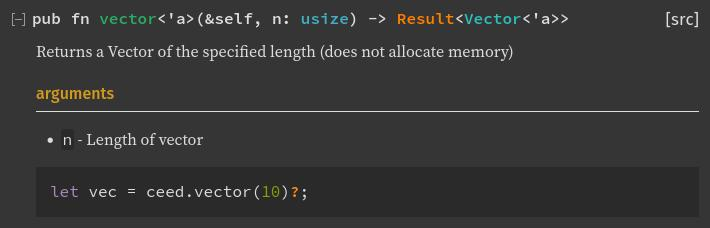
\includegraphics[height=3.25cm]{libCEEDRustVecDoc}

\end{center}
\end{frame}

%-------------------------------------------------------------------------------

\begin{frame}[fragile]
\begin{center}
\frametitle{Lost in Translation}

Passive vectors can be mutated by operators\\

~\\

{\footnotesize
\begin{lstlisting}[language=Rust, style=boxedRust]
// Mass operator
let qf_mass = ceed.q_function_interior_by_name("MassApply")?;
let op_mass = ceed
     .operator(&qf_mass, QFunctionOpt::None, QFunctionOpt::None)?
     .field("u", &ru, &bu, VectorOpt::Active)?
     .field("qdata", &rq, BasisOpt::Collocated, &qdata)?
     .field("v", &ru, &bu, VectorOpt::Active)?
     .check()?;

v.set_value(0.0)?;
op_mass.apply(&u, &mut v)?;
\end{lstlisting}
}

~\\

If {\color[rgb]{0, 0, 0.75} \lstinline[basicstyle=\ttfamily, columns=spaceflexible]{"qdata"}} was an output, the operator could mutate the underlying data without the Rust compiler knowing
\end{center}
\end{frame}

%-------------------------------------------------------------------------------
\section{petsc-rs}
%-------------------------------------------------------------------------------

\begin{frame}
\begin{center}
\frametitle{PETSc - the Portable, Extensible Toolkit for Scientific Computation}

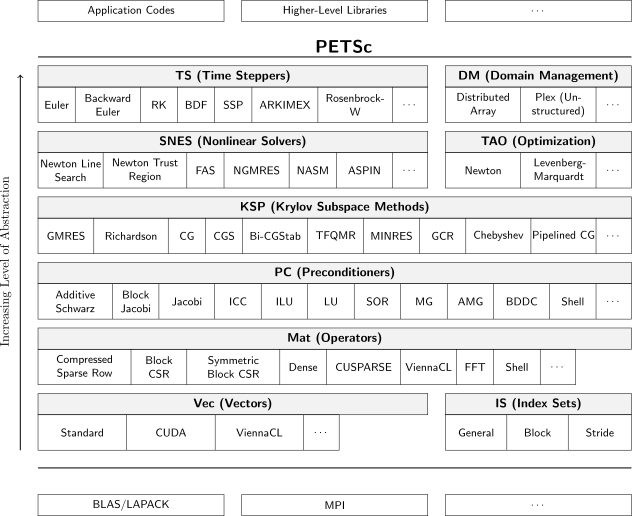
\includegraphics[height=6.5cm]{PETScAPI}\cite{petsc}

\end{center}
\end{frame}

%-------------------------------------------------------------------------------

\begin{frame}
\begin{center}
\frametitle{petsc-rs}

\href{https://lib.rs/crates/petsc}{https://lib.rs/crates/petsc}\\

\href{https://gitlab.com/petsc/petsc-rs}{https://gitlab.com/petsc/petsc-rs}\\

~\\

\begin{itemize}

\item Attempt to maintain flexibility of C API\\

~\\

\item Wider range of additional objects to manage borrowed access\\

~\\

\item Currently incomplete shell object support\\

\end{itemize}

\end{center}
\end{frame}

%-------------------------------------------------------------------------------

\begin{frame}[fragile]
\begin{center}
\frametitle{High Level Abstractions - Matrix assembly}

{\footnotesize
\begin{lstlisting}[language=Rust, style=boxedRust]
let n = 5;
let mut mat = petsc.mat_create()?;
mat.set_sizes(None, None, n as usize, n as usize)?;
mat.set_from_options()?;
mat.set_up()?;

// Stencil (-1, 2, -1)
let v = [Scalar::from(-1.0), Scalar::from(2.0), Scalar::from(-1.0)];
mat.assemble_with_batched(
    (0..n)
        .map(|i| {
            if i == 0 { ([i], [-1, i, i + 1], &v) }
            else if i == n - 1 { ([i], [i - 1, i, -1], &v) }
            else { ([i], [i - 1, i, i + 1], &v) }
        }),
    InsertMode::INSERT_VALUES,
    MatAssemblyType::MAT_FINAL_ASSEMBLY,
)?;
\end{lstlisting}
}

\end{center}
\end{frame}

%-------------------------------------------------------------------------------

\begin{frame}
\begin{center}
\frametitle{Lost in Translation - Part II}

\begin{itemize}

\item PETSc objects have bi-directional data ownership\\

~\\

\item Compiler can't reliably reason about complex lifetimes\\

~\\

\item The libCEED wrapper provides performance portable matrix-free finite element operators\\

~\\

\item The PETSc wrapper is a more complex ongoing challenge\\

\end{itemize}

\end{center}
\end{frame}

%-------------------------------------------------------------------------------
\section{Summary}
%-------------------------------------------------------------------------------

\begin{frame}
\begin{center}
\frametitle{Rust for HPC}

\begin{itemize}

\item Rust provides high performance with modern tooling and ergonomic language features\\

~\\

\item We looked at the libCEED and PETSc Rust wrappers\\

~\\

\item The libCEED wrapper provides performance portable matrix-free finite element operators\\

~\\

\item The PETSc wrapper is a more complex ongoing challenge\\

\end{itemize}

~\\

\bf{Rust is ready for HPC - but it requires rethinking your design!}

\end{center}
\end{frame}

%-------------------------------------------------------------------------------

\begin{frame}
\begin{center}
\frametitle{Future Work}

\begin{itemize}

\item Expand PETSc Rust wappers\\

~\\

\item Native Rust libCEED QFunctions for GPU\\

~\\

\item PETSc + libCEED Rust examples\\

~\\

\item Clarify inner mutability vs interface level mutability across FFI barrier\\

~\\

\item Disentangling object lifetimes\\

\end{itemize}

\end{center}
\end{frame}

%-------------------------------------------------------------------------------

\begin{frame}[noframenumbering]
\titlepage % Print the title page
\end{frame}

\begin{frame}[noframenumbering,allowframebreaks]
\bibliographystyle{plain} % or "siam", or "alpha", etc.
\bibliography{references} % Bib database in "refs.bib"
\end{frame}

\begin{frame}[noframenumbering]
\titlepage % Print the title page
\end{frame}

%-------------------------------------------------------------------------------

\end{document}

%-------------------------------------------------------------------------------
